 \documentclass{beamer}
  \usepackage[utf8]{inputenc}
  \usetheme{Warsaw}
  %\graphicspath{tabularx}
  
  \usepackage{graphicx}
\usepackage{epsfig}
\usepackage{amssymb}
\usepackage{amsmath}
\usepackage{array}
\usepackage{subfig}
\usepackage{multicol}
\usepackage{caption}
\usepackage{listings}
\usepackage{algorithm}
\usepackage{algorithmic}
\usepackage{array,multirow,makecell}

  \title{Stéganographie \& Stéganalyse : Démonstration}
  \author{StegX}
  \institute{UFR des Sciences Versailles - L3 Informatique}
  \date{1er Juin 2018}

  \begin{document}

  \begin{frame}
  \titlepage
  \end{frame}
  
  \section{Que propose StegX ?}
    
	\begin{frame}
  
\includegraphics[scale=0.3]{pictures/bilan_0}
  \end{frame}
  
  \subsection{Interfaces}
  
  \begin{frame}
  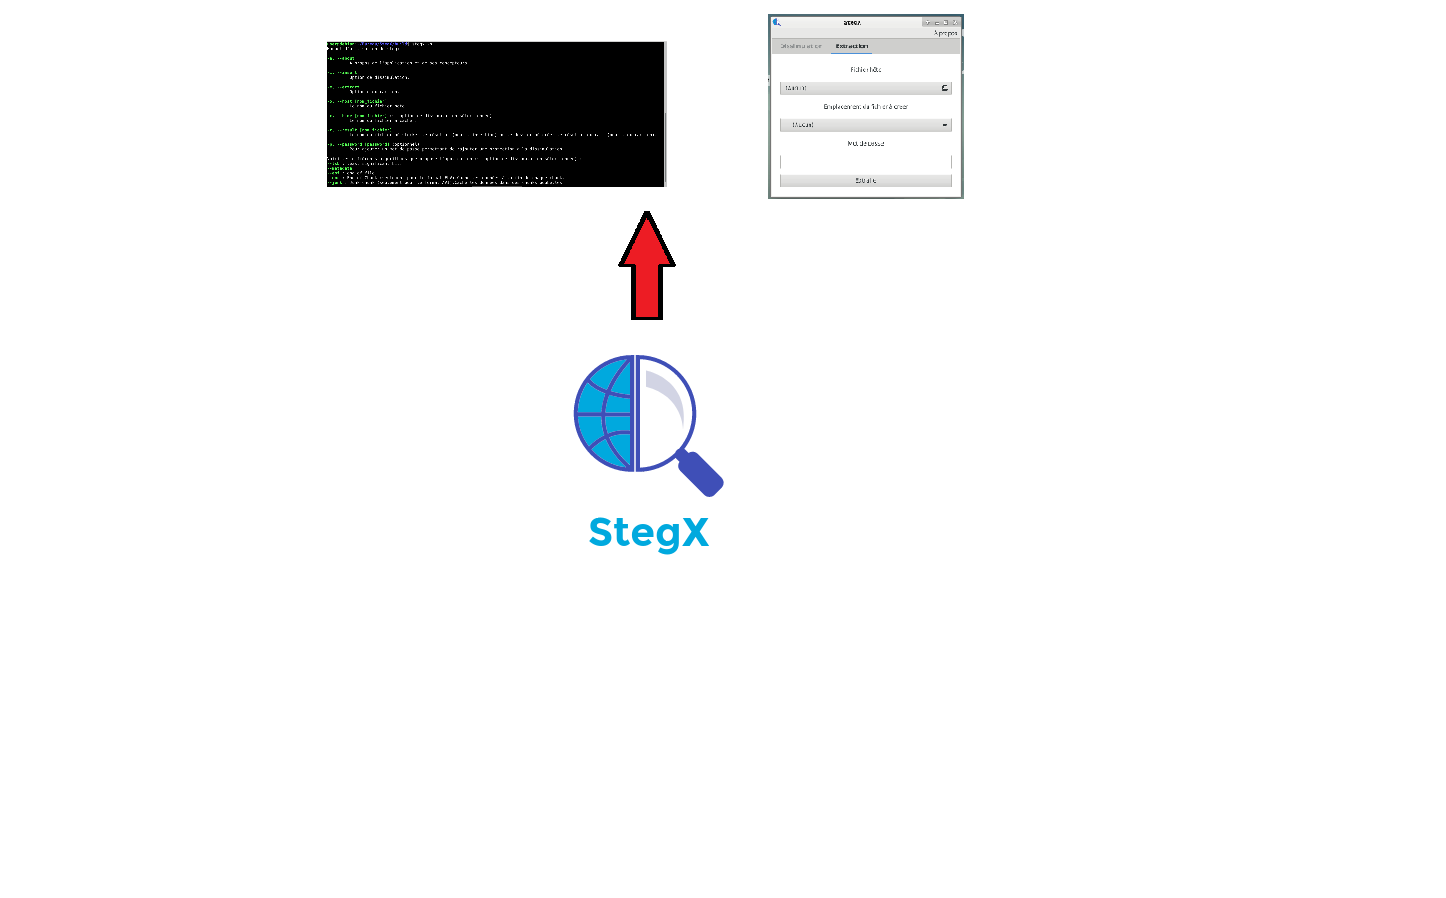
\includegraphics[scale=0.3]{pictures/bilan_1}
  \end{frame}
  
  \subsection{Multi-plateforme}
  
  \begin{frame}
  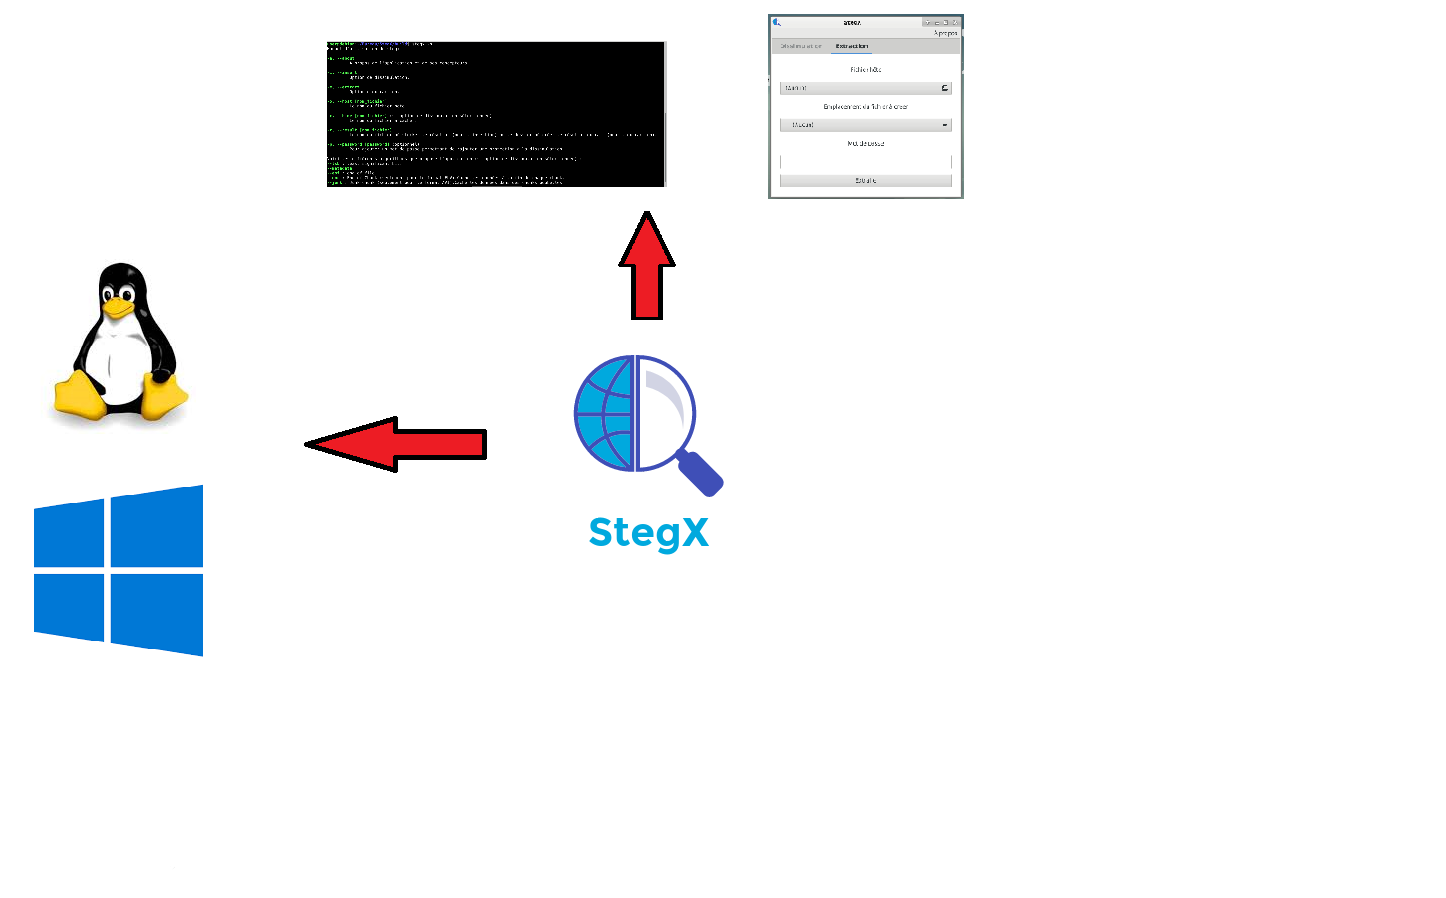
\includegraphics[scale=0.3]{pictures/bilan_2}
  \end{frame}
  
  \subsection{3 types dont 6 formats}
  
  \begin{frame}
  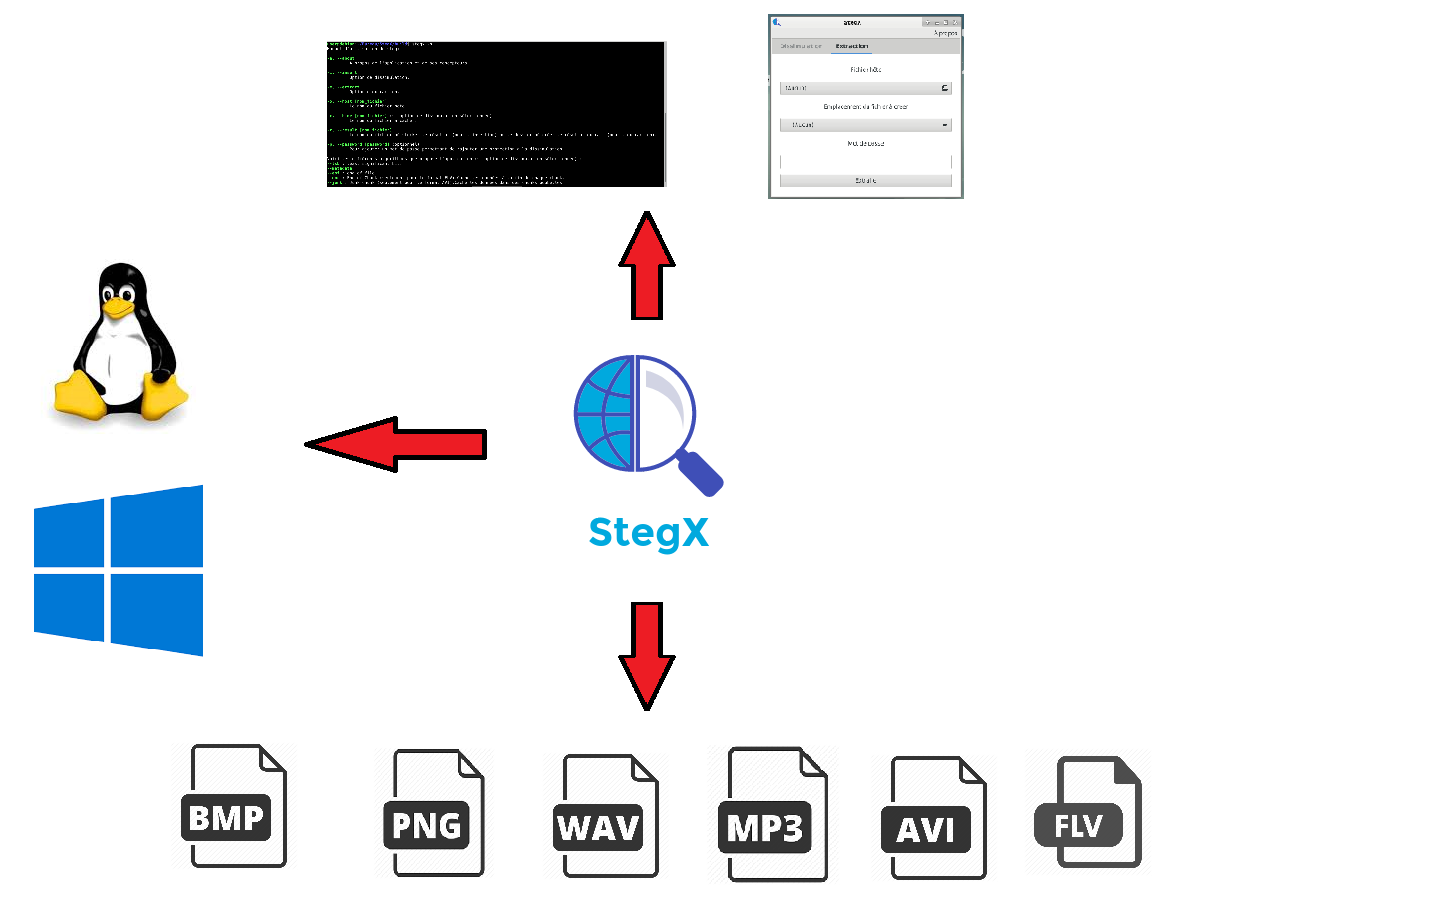
\includegraphics[scale=0.3]{pictures/bilan_3}
  \end{frame}
  
  \subsection{5 algorithmes de stéganographie}
  
  \begin{frame}
  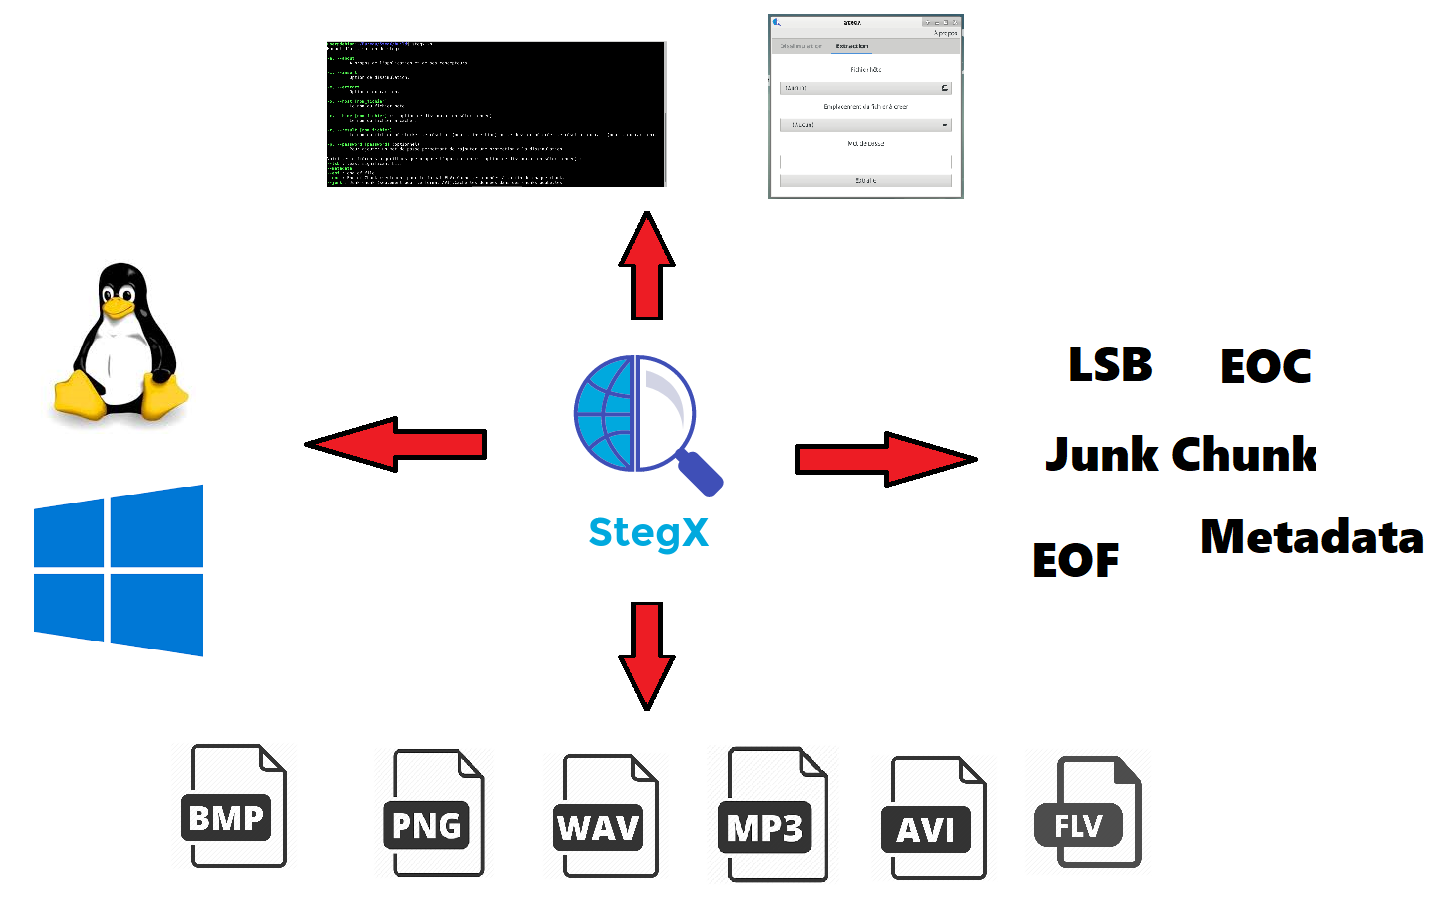
\includegraphics[scale=0.3]{pictures/bilan_4}
  \end{frame}
  
  \section{Quels algos pour quels formats ?}
  
  \begin{frame}
  
	Le produit répond bien aux objectifs et propose ces algorithmes pour 
	ces formats : 
\newline

\begin{tabular}{|c|c|c|c|c|c|}
  \hline
  \multirow{2}*{\textbf{Format}} & \multicolumn{5}{c|}{\textbf{Algorithmes proposés}} \\
   \cline{2-6}
    & \textbf{LSB} & \textbf{EOF} & \textbf{Metadata} 
    &\textbf{EOC} & \textbf{Junk Chunk} \\
  \hline
  \textbf{BMP} & \textbf{\checkmark} & \textbf{\checkmark} & \textbf{\checkmark} &  & \\
  \hline      
  \textbf{PNG} &  & \textbf{\checkmark} & \textbf{\checkmark} & & \\
  \hline
  \textbf{WAV} & \textbf{\checkmark} & \textbf{\checkmark} & & & \\
  \hline 
  \textbf{MP3} & \textbf{\checkmark} & \textbf{\checkmark} & & & \\
  \hline 
  \textbf{AVI} & & & & & \textbf{\checkmark}\\
  \hline
  \textbf{FLV} & & \textbf{\checkmark} & & \textbf{\checkmark} & \\
  \hline
\end{tabular}

\end{frame}
  
  \end{document}
